

\tikzset{every picture/.style={line width=0.75pt}} %set default line width to 0.75pt        

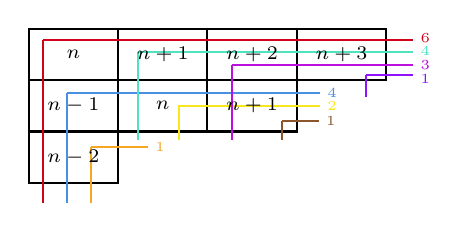
\begin{tikzpicture}[x=0.75pt,y=0.75pt,yscale=-1,xscale=1]
	%uncomment if require: \path (0,91); %set diagram left start at 0, and has height of 91
	
	%Shape: Rectangle [id:dp8815777045687874] 
	\draw   (231,3.2) -- (274.06,3.2) -- (274.06,27.97) -- (231,27.97) -- cycle ;
	%Shape: Rectangle [id:dp5991219333253064] 
	\draw   (274.06,3.2) -- (317.11,3.2) -- (317.11,27.97) -- (274.06,27.97) -- cycle ;
	%Shape: Rectangle [id:dp045704656972568536] 
	\draw   (317.11,3.2) -- (360.17,3.2) -- (360.17,27.97) -- (317.11,27.97) -- cycle ;
	%Shape: Rectangle [id:dp9709748524524378] 
	\draw   (360.17,3.2) -- (403.22,3.2) -- (403.22,27.97) -- (360.17,27.97) -- cycle ;
	%Shape: Rectangle [id:dp2596405378230242] 
	\draw   (231,27.97) -- (274.06,27.97) -- (274.06,52.73) -- (231,52.73) -- cycle ;
	%Shape: Rectangle [id:dp42226610658689956] 
	\draw   (274.06,27.97) -- (317.11,27.97) -- (317.11,52.73) -- (274.06,52.73) -- cycle ;
	%Shape: Rectangle [id:dp4187316025482162] 
	\draw   (317.11,27.97) -- (360.17,27.97) -- (360.17,52.73) -- (317.11,52.73) -- cycle ;
	%Shape: Rectangle [id:dp5305320625060379] 
	\draw   (231,52.73) -- (274.06,52.73) -- (274.06,77.49) -- (231,77.49) -- cycle ;
	%Straight Lines [id:da06952631342029836] 
	\draw [color={rgb, 255:red, 208; green, 2; blue, 27 }  ,draw opacity=1 ]   (237.87,8.48) -- (237.87,87.2) ;
	%Straight Lines [id:da009607264963725326] 
	\draw [color={rgb, 255:red, 208; green, 2; blue, 27 }  ,draw opacity=1 ]   (237.87,8.48) -- (416.31,8.48) ;
	%Straight Lines [id:da7757112780471731] 
	\draw [color={rgb, 255:red, 74; green, 144; blue, 226 }  ,draw opacity=1 ]   (249.46,34.22) -- (249.46,87.2) ;
	%Straight Lines [id:da7936647011909119] 
	\draw [color={rgb, 255:red, 74; green, 144; blue, 226 }  ,draw opacity=1 ]   (249.46,34.22) -- (371.37,34.22) ;
	%Straight Lines [id:da2080337074460996] 
	\draw [color={rgb, 255:red, 245; green, 166; blue, 35 }  ,draw opacity=1 ]   (261.04,60.31) -- (261.04,87.2) ;
	%Straight Lines [id:da1672284401195936] 
	\draw [color={rgb, 255:red, 245; green, 166; blue, 35 }  ,draw opacity=1 ]   (261.04,60.31) -- (288.56,60.31) ;
	%Straight Lines [id:da9072636327703945] 
	\draw [color={rgb, 255:red, 80; green, 227; blue, 194 }  ,draw opacity=1 ]   (283.62,14.27) -- (283.62,56.84) ;
	%Straight Lines [id:da23576145614184396] 
	\draw [color={rgb, 255:red, 80; green, 227; blue, 194 }  ,draw opacity=1 ]   (283.62,14.27) -- (416.31,14.27) ;
	%Straight Lines [id:da13302174297805824] 
	\draw [color={rgb, 255:red, 248; green, 231; blue, 28 }  ,draw opacity=1 ]   (303.31,40.62) -- (303.31,56.84) ;
	%Straight Lines [id:da18353762508780203] 
	\draw [color={rgb, 255:red, 248; green, 231; blue, 28 }  ,draw opacity=1 ]   (303.04,40.62) -- (371.37,40.62) ;
	%Straight Lines [id:da18141605076501444] 
	\draw [color={rgb, 255:red, 139; green, 87; blue, 42 }  ,draw opacity=1 ]   (353.11,47.57) -- (353.11,56.8) ;
	%Straight Lines [id:da4919198143241954] 
	\draw [color={rgb, 255:red, 139; green, 87; blue, 42 }  ,draw opacity=1 ]   (353.11,47.57) -- (370.79,47.57) ;
	%Straight Lines [id:da4333346176137032] 
	\draw [color={rgb, 255:red, 189; green, 16; blue, 224 }  ,draw opacity=1 ]   (328.79,20.64) -- (328.79,56.8) ;
	%Straight Lines [id:da4927197010903921] 
	\draw [color={rgb, 255:red, 189; green, 16; blue, 224 }  ,draw opacity=1 ]   (328.79,20.64) -- (416.31,20.64) ;
	%Straight Lines [id:da1285065636768843] 
	\draw [color={rgb, 255:red, 144; green, 19; blue, 254 }  ,draw opacity=1 ]   (393.65,25.57) -- (393.65,35.99) ;
	%Straight Lines [id:da850577775142418] 
	\draw [color={rgb, 255:red, 144; green, 19; blue, 254 }  ,draw opacity=1 ]   (393.65,25.57) -- (416.31,25.57) ;
	
	
	% Text Node
	\draw (252.53,15.58) node  [font=\scriptsize]  {$n$};
	% Text Node
	\draw (295.58,15.58) node  [font=\scriptsize]  {$n+1$};
	% Text Node
	\draw (252.53,40.35) node  [font=\scriptsize]  {$n-1$};
	% Text Node
	\draw (338.64,15.58) node  [font=\scriptsize]  {$n+2$};
	% Text Node
	\draw (295.58,40.35) node  [font=\scriptsize]  {$n$};
	% Text Node
	\draw (338.64,40.35) node  [font=\scriptsize]  {$n+1$};
	% Text Node
	\draw (381.69,15.58) node  [font=\scriptsize]  {$n+3$};
	% Text Node
	\draw (252.53,65.11) node  [font=\scriptsize]  {$n-2$};
	% Text Node
	\draw (290.56,60.31) node [anchor=west] [inner sep=0.75pt]  [font=\tiny,color={rgb, 255:red, 245; green, 166; blue, 35 }  ,opacity=1 ]  {$1$};
	% Text Node
	\draw (372.79,47.57) node [anchor=west] [inner sep=0.75pt]  [font=\tiny,color={rgb, 255:red, 139; green, 87; blue, 42 }  ,opacity=1 ]  {$1$};
	% Text Node
	\draw (418.31,27.57) node [anchor=west] [inner sep=0.75pt]  [font=\tiny,color={rgb, 255:red, 144; green, 19; blue, 254 }  ,opacity=1 ]  {$1$};
	% Text Node
	\draw (373.37,40.62) node [anchor=west] [inner sep=0.75pt]  [font=\tiny,color={rgb, 255:red, 248; green, 231; blue, 28 }  ,opacity=1 ]  {$2$};
	% Text Node
	\draw (373.37,34.22) node [anchor=west] [inner sep=0.75pt]  [font=\tiny,color={rgb, 255:red, 74; green, 144; blue, 226 }  ,opacity=1 ]  {$4$};
	% Text Node
	\draw (418.31,20.64) node [anchor=west] [inner sep=0.75pt]  [font=\tiny,color={rgb, 255:red, 189; green, 16; blue, 224 }  ,opacity=1 ]  {$3$};
	% Text Node
	\draw (418.31,14) node [anchor=west] [inner sep=0.75pt]  [font=\tiny,color={rgb, 255:red, 80; green, 227; blue, 194 }  ,opacity=1 ]  {$4$};
	% Text Node
	\draw (418.31,7.48) node [anchor=west] [inner sep=0.75pt]  [font=\tiny,color={rgb, 255:red, 208; green, 2; blue, 27 }  ,opacity=1 ]  {$6$};
	
	
\end{tikzpicture}